
\begin{figure}
  \setlength{\fboxsep}{0pt} % box tighlty around text
  \begin{subfigure}{0.48\textwidth}
    \fbox{% frame
      \adjustbox{valign=B}{% margins
        \resizebox{\textwidth}{!}{% scale
          \lstinputlisting[
            basicstyle=\scriptsize\sffamily,
            language=sparql, numbers=none, columns=flexible,
            commentstyle=\color{Gray!70},
            showstringspaces=false]{
            figures/query-q1-j2-no-star.rq
      } } } }
    \caption{\label{fig:q1-j2-1hop}Query $Q_e$: All cycling races of Central America along
      with their respective country.}
  \end{subfigure}
  \hfill
  \begin{subfigure}{0.48\textwidth}
    \fbox{%
      \resizebox{\textwidth}{!}{% scale
        
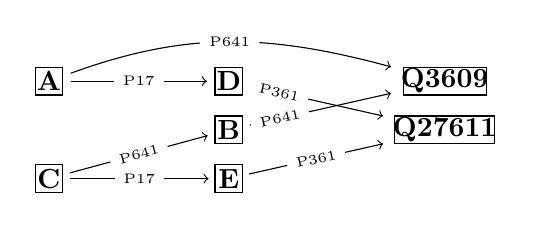
\begin{tikzpicture}

  \thickmuskip=0mu
  \medmuskip=0mu
  \thinmuskip=0mu

  \newcommand\X{65pt}
  \newcommand\Y{-17.6pt}
  \newcommand\PREDICATE{\tiny}
  
  \draw (0, 0) node(A){\textbf{A}} +(-5pt, -5pt) rectangle +(5pt, 5pt);
  \draw (\X, 0) node(D){\textbf{D}} +(-5pt, -5pt) rectangle +(5pt, 5pt);
  \draw (2.2*\X, 0) node(Q3609){\textbf{Q3609}} +(-15pt, -5pt) rectangle +(15pt, 5pt);

  \draw (\X, \Y) node(B){\textbf{B}} +(-5pt, -5pt) rectangle +(5pt, 5pt);
  \draw (2.2*\X, \Y) node(Q27611){\textbf{Q27611}} +(-18pt, -5pt) rectangle +(18pt, 5pt);
  \draw (0, 2*\Y) node(C){\textbf{C}} +(-5pt, -5pt) rectangle +(5pt, 5pt);
  \draw (1*\X, 2*\Y) node(E){\textbf{E}} +(-5pt, -5pt) rectangle +(5pt, 5pt);
  

  \draw[->] (A) -- node[fill=white, font=\PREDICATE]{P17} (D);
  \draw[->] (C) -- node[fill=white, sloped, font=\PREDICATE]{P641} (B);
  \draw[->] (C) -- node[fill=white, sloped, font=\PREDICATE]{P17} (E);
  \draw[->] (B) -- node[fill=white, sloped, font=\PREDICATE, xshift=-1.5em]{P641} (Q3609);
  \draw[->] (E) -- node[fill=white, sloped, font=\PREDICATE]{P361} (Q27611);
  \draw[->] (D) -- node[fill=white, sloped, font=\PREDICATE, xshift=-1.4em]{P361} (Q27611);
  \draw[->] (A) to[out=20, in=165] node[fill=white,sloped, font=\PREDICATE]{P641} (Q3609);
  
  

\end{tikzpicture}

    }}
    % \includegraphics[width=\textwidth]{figures/graph-g1.png}
    \caption{RDF Graph $G_1$: $A$, $B$, and $C$ are cycling sports; $D$ and $E$
      are countries of Central America.}
  \end{subfigure}
  \caption{\label{fig:random_walks_example}Query $Q_e$  evaluated on the RDF graph $G_1$ from \cite{10.1007/978-3-031-33455-9_3}.
    \TODO{Better caption}}
\end{figure}

\section{\NAME: RAndom Walks for Apache Jena}

\paragraph{Sampling principles.}

\NAME is based on WanderJoin\cite{li2019wanderjoin}.
Let $Q$ be a SPARQL conjunctive query, and $J = \langle tp_1, ..., tp_n \rangle$ be
the join order used to perform random walks. A random walk
$\gamma_i = \langle t_1, ..., t_n\rangle$ is computed over
an RDF graph $G$ by randomly picking $t_1$ in $\llbracket tp_1 \rrbracket_G$,
and each subsequent $t_i$ ($i > 1$) in $\llbracket t_{i-1} \bowtie tp_i \rrbracket_G$.
Once computed, the cardinality of $Q$ is estimated as the inverse probability
of sampling $\gamma_i$, i.e. $P(\gamma_i)^{-1}$, with $P(\gamma_i) = |\llbracket tp_1 \rrbracket_G|^{-1} \prod_{i=2}^{n}
|\llbracket t_{i-1} \bowtie tp_i \rrbracket_G|^{-1}$.

For instance, let us consider the query $Q_e$ and the RDF graph $G_1$
depicted in Figure~\ref{fig:random_walks_example}. Following the join order $tp_3,tp_2,tp_1$, the random walk 
$\gamma_1$ is computed as follow:

% \begin{center}
  \begin{small}
    \begin{tabular}{l|lll}
      $tp_3$ & draw  $t_1$ &$= (\textbf{A}, P641, Q3609)$ & $\in \llbracket (?x1, P641, Q3609) \rrbracket_{G_1}$ \\
      $tp_2$ & draw  $t_2$ &$= (A, P17, \textbf{D})$ & $ \in \llbracket (\textbf{A}, P17, ?x3) \rrbracket_{G_1}$  \\
      $tp_1$ & draw  $t_3$ &$= (D, P361, Q27611)$ & $\in \llbracket (\textbf{D}, P361, Q27611) \rrbracket_{G_1}$  
    \end{tabular}
  \end{small} 
% \end{center}

\noindent The cardinality of $Q_e$ is then estimated as the inverse
probability of sampling $\gamma_1$:
\begin{small}

\noindent\begin{tabular}{ll}
    $P(\gamma_1)^{-1}$  &$=  |\llbracket (?x1, P641, Q3609) \rrbracket_{G_1}| \times
                          |\llbracket (\textbf{A}, P17, ?x3) \rrbracket_{G_1}| \times
                          |\llbracket (\textbf{D}, P361,
                          Q27611) \rrbracket_{G_1}| $ \\
                      &$=  2 \times 1 \times 1 = 2$
\end{tabular}
\end{small}

\noindent Of course, a random walk may fail if it becomes impossible to sample $t_i$ for
some $i \leq n$. In this case, its probability $P(\gamma_i)$ of being sampled is 0.
For instance, if $t_1 = (B, P641, Q3609)$ is picked in
$\llbracket (?x1, P641, Q3609) \rrbracket_{G_1}$
instead of $(A, P641, Q3609)$, then the random walk fails because
$\llbracket (B, P17, ?x3) \rrbracket_{G_1} = \emptyset$.
%
To improve the quality of estimates, instead of computing only one random
walk, a set $\Gamma = \langle \gamma_1, ..., \gamma_k \rangle$ of $k$ random walks is computed,
and the cardinality of the query is estimated as $card(\Gamma) =
|\Gamma|^{-1}\sum_{i=1}^{|\Gamma|} P(\gamma_i)^{-1}$.


\paragraph{\NAME in action}


% ?x1 <http://www.wikidata.org/prop/direct/P31> <http://www.wikidata.org/entity/Q5> . ?x2 <http://www.wikidata.org/prop/direct/P31> <http://www.wikidata.org/entity/Q5> . ?x1 <http://www.wikidata.org/prop/direct/P569> ?x3 . ?x2 <http://www.wikidata.org/prop/direct/P569> ?x3 . ?x1 <http://www.wikidata.org/prop/direct/P570> ?x4 . ?x2 <http://www.wikidata.org/prop/direct/P570> ?x4 . 

 \begin{figure*}
   \centering
   \includegraphics[width=0.85\textwidth]{figures/raw_screenshot.png}
   \caption{\label{fig:raw_screenshot}User interface of \NAME providing useful insights on the query.}
 \end{figure*}

%\paragraph{Target audience.}
%Researchers and practitioners in need of sampling services over RDF
%knowledge graphs. \TODO{In fields.}

 As a motivating example, we rely on the query $Q_{604}$ of
 WDBench~\cite{angles2022wdbench} presented in the
 figure~\ref{fig:raw_screenshot}. This query are looking for people
 with the same birth and death date. This query returns ~25M results,
 time-out on the public Wikidata SPARQL endpoint, and takes more than
 2 hours to execute on JENA. However, in 35 seconds \NAME estimates the
 cardinality of $Q_{604}$ around 26 millions of results more or less 3
 millions and returns 1434 random results.

 
% \paragraph{Web interface.}
 Figure~\ref{fig:raw_screenshot} presents the user interface
 exploiting \NAME's random walks. The top part of the figure shows
 where the users type their queries. The bottom panel displays the
 random walks $\gamma_i$ with $P(\gamma_i))$ ie. all displayed random
 walks failed.  The left panel presents the evolution of cardinality
 estimation and confidence interval when the number of random walks
 increases. As we can see, the cardinality estimation converges to the
 real cardinality.

 The right panel display the join order $J$ with number of random
 walks that reach the triple pattern ie. for 100000 random walks
 launched on $quad_1$, only 1434 reached $quad_6$.

 By pressing the play button, it asks the server for random walks on
 this whole BGP. When the server reaches a configurable threshold of
 $10 000$ random walks, or $60s$ execution time, it returns its
 results. By repeating the operation, results are merged iteratively
 in a pay-as-you-go fashion hence displaying more accurate
 information. Figure~\ref{fig:raw_screenshot} shows that over $10$
 iterations, \NAME performed $100k$ random walks but only $1434$
 actual successes.

 % Yet, the bottom left figure provides an estimation
 % of the number of results over the number of random walks with
 % confidence intervals. The bottom right figure provides the estimated
 % number of intermediate results along with the number of random walks
 % that reached each triple/quad pattern.  Finally, the bottom part
 % shows both failed and succeeded random walks along with the
 % probability that they were chosen at execution time.

% \paragraph{Getting insights on timed out WDBench queries.}
% A few queries of WDBench fail to execute under the 60 seconds mark,
% providing nothing whatsoever. We execute these queries using \NAME and
% show that, with as little as 1 second, we retrieve interesting
% insights on the query plan that may help optimizers to perform their
% join ordering. We also get a rough approximation of the number of
% results that we improve by executing the query for additional seconds.
% The plotted curve converges towards the actual cardinality of the query.



% %%% Local Variables:
% %%% mode: latex
% %%% TeX-master: "../paper.tex"
% %%% End:
